\documentclass[tikz,border=3pt]{standalone}
\usepackage[utf8]{inputenc}
\usepackage[T1]{fontenc}
\usepackage{lmodern}
\renewcommand{\familydefault}{\sfdefault}
\usepackage{sansmath}\sansmath
\usepackage{chemfig}
\usepackage{pgfplots}\pgfplotsset{compat=1.18,/pgf/number format/use comma,/pgf/number format/1000 sep={.}}
\usetikzlibrary{arrows.meta,calc,positioning,decorations.pathmorphing,patterns}
% paleta del sitio
\definecolor{nar}{HTML}{E8680C}\definecolor{narc}{HTML}{FFB35C}\definecolor{hielo}{HTML}{FFF3E8}
\definecolor{tinta}{HTML}{1D1D1F}\definecolor{gris}{HTML}{6E6E73}\definecolor{lila}{HTML}{7C5CF0}
\definecolor{azul}{HTML}{2F6FD6}\definecolor{menta}{HTML}{17A673}\definecolor{coral}{HTML}{E8342A}
\begin{document}
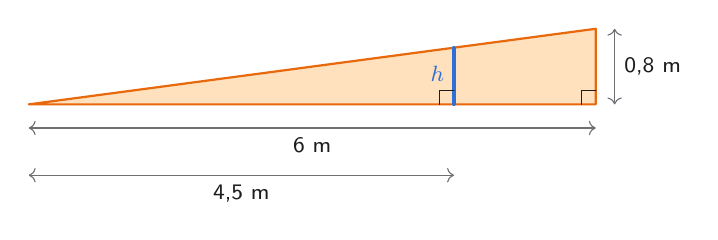
\begin{tikzpicture}[font=\small,x=0.6cm,y=0.6cm,line cap=round,line join=round,step={(1,1)}]
\filldraw[fill=narc!40,draw=nar,thick] (0,0)--(12,0)--(12,1.6)--cycle;
\draw[azul,very thick] (9,0)--(9,1.2);
\draw[tinta] (11.7,0)--(11.7,0.3)--(12,0.3); \draw[tinta] (8.7,0)--(8.7,0.3)--(9,0.3);
\draw[<->,gris] (0,-0.5)--(12,-0.5) node[midway,below,font=\footnotesize,text=tinta] {6 m};
\draw[<->,gris] (0,-1.5)--(9,-1.5) node[midway,below,font=\footnotesize,text=tinta] {4,5 m};
\draw[<->,gris] (12.4,0)--(12.4,1.6) node[midway,right,font=\footnotesize,text=tinta] {0,8 m};
\node[left,font=\footnotesize,text=azul] at (9,0.65) {$h$};
\end{tikzpicture}
\end{document}
